\chapter{Introdução}
\label{cha:introducao}

O intercâmbio de informações é um tema chave logística moderna. A logística da informação lida com o fluxo de informações entre humanos e/ou máquinas dentro ou entre organizações \cite{haftor2011information}, que se agrupam formando uma rede de criação de valor por meio de informações.

Com o cenário de comércio em um mundo intrinsecamente globalizado, as cadeias de suprimentos (CS) e suas interdependências tornam-se mais complexas. O compartilhamento de informações entre os elos da CS, portanto, é uma forma de dar visibilidade sobre o atual estado de itens percorrendo a cadeia.

Quando se trata de informações relativas a um produto, o conceito de Memória Digital do Produto (MDP) pode ser utilizado como forma de coletar, armazenar e fornecer informações. A MDP se refere a sistemas que permitem a coleta de dados em todas as fases do ciclo de vida do produto para distribuição e/ou análise \cite{wahlster2007digitalmemory}. Os dados de interesse do produto se relacionam a qualquer fase de sua cadeia de valor, o que abrange dados de produção, montagem, distribuição (transporte) \cite{brandherm2011productmemory}, padrões de uso pelo cliente final, etc.

O compartilhamento destas informações geradas a partir dos dados favorece o desenvolvimento de novas versões do próprio produto e funciona também como um elo permanente entre o fornecedor e o cliente no pós-venda, permitindo que o produto mantenha atualizações e quaisquer outras melhorias instantaneamente.

Tais conceitos de compartilhamento de informações de produtos por meio da MDP se encaixam na proposta da Indústria 4.0 (I4.0), que tem como fundamentos a inserção de novas tecnologias com o propósito de oferecer um alto nível de automação e intercâmbio de informações entre equipamentos e produtos \cite{lasi2014industryfour}.

Portanto, surge na I4.0 oportunidades para a criação de novas soluções centradas no amplo compartilhamento de informações ao longo da cadeia de suprimentos, além de novas metodologias para a extração e análise dessas informações para desenvolvimento de outros produtos aperfeiçoados.

A Logística da Informação e a MDP, mencionados anteriormente, são intrinsecamente relacionados à I4.0, que por sua vez faz o uso extensivo de conhecimentos e técnicas das área de Gestão da Informação (GI) e Tecnologia de Informação e Comunicação (TIC).

A Indústria 4.0 surgiu a partir da crescente integração das Tecnologias da Informação e Comunicação (TIC) às cadeias de valor industriais, criando as bases para a próxima revolução industrial \cite{hermann2016design}. Essa mudança de paradigma na indústria se refere às recentes modificações em relação às tecnologias de manufatura, que passam a proporcionar um alto nível de automação e intercâmbio de informações entre equipamentos, produtos e demais atores em um ambiente de manufatura \cite{lasi2014industryfour}.

O nome Indústria 4.0 (I4.0) se dá ao fato de ser considerada a quarta maior revolução com relação à tecnologia de produção industrial, sendo as ``revoluções industriais'' consideradas evoluções tecnológicas que levaram a grandes mudanças no paradigma de produção, tal histórico de revoluções no campo da indústria é ilustrado na \autoref{fig:i4}.

\begin{figure}[htb]
	\centering
	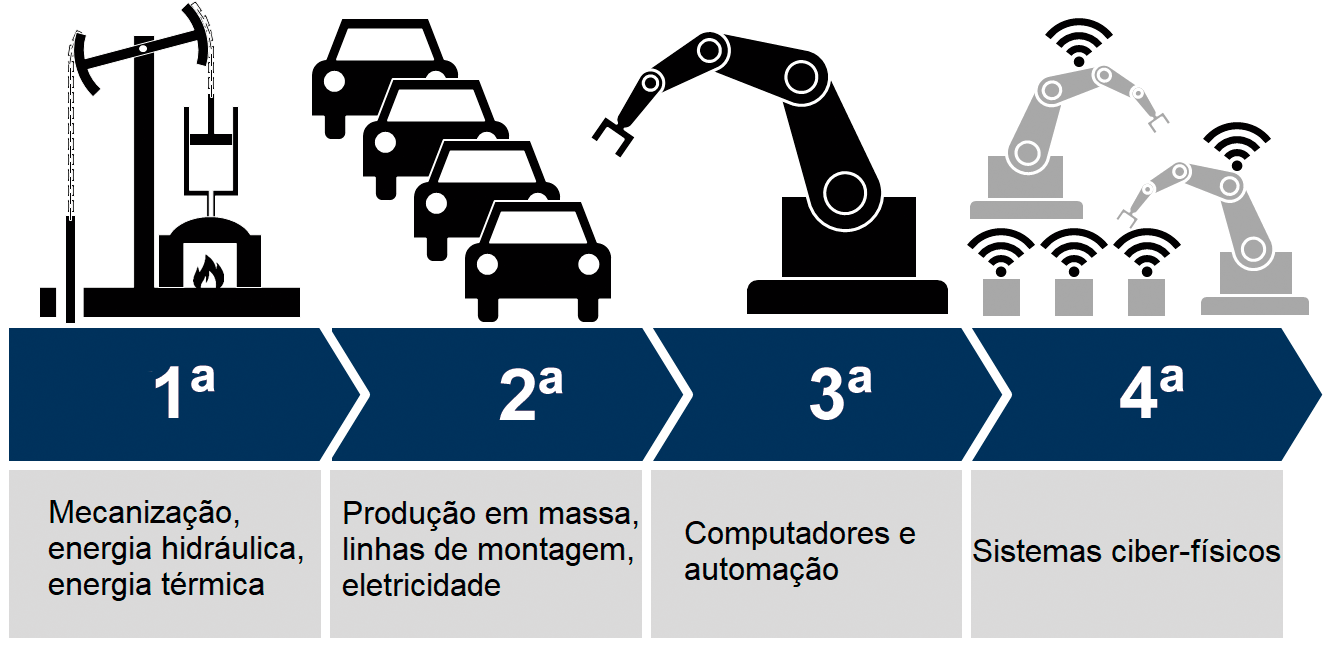
\includegraphics[width=1\textwidth]{i4.png}
	\caption{As revoluções industriais.}
	\label{fig:i4}
	\fonte{\citeonline{lasi2014industryfour} (adaptado).}
\end{figure}

Tais modificações são essenciais devido às novas necessidades da própria indústria e às mudanças de padrões de consumo do mercado. Isto acarreta transformações no cenário operacional destas indústrias. Algumas das causas dessas mudanças operacionais são \cite{lasi2014industryfour}:

\begin{itemize}

	\item Períodos de desenvolvimento curtos: Os períodos de desenvolvimento e inovação de produtos estão sendo reduzidos. A alta capacidade de inovação está se tornando um fator de sucesso para muitas empresas (\textit{Time to market});

	\item Individualização sob demanda: Os compradores passam a definir as condições de compra. Essa tendência leva a uma crescente individualização de produtos com características altamente personalizadas e, em casos extremos, a produtos individuais;

	\item Flexibilidade: Devido à individualização sob demanda, novas estruturas e organizações na indústria são essenciais para a fabricação de produtos com alto grau de personalização. É necessária uma maior flexibilidade no desenvolvimento do produto, especialmente na produção;

	\item Descentralização: Para lidar com condições específicas de cada produto, são necessários procedimentos mais rápidos de tomada de decisão. Para isso, as hierarquias organizacionais precisam ser reduzidas, dando ao produto maior independência sobre seu próprio processo de fabricação;

	\item Eficiência de recursos: A maior eficiência sobre o uso dos recursos sempre é algo desejável, porém sua importância se intensifica com as tendências de aumento dos preços dos recursos, bem como a mudança social no contexto de aspectos ecológicos. Isto exige um foco mais intensivo em sustentabilidade, o que decorre em uma maior racionalidade (ou eficiência) na utilização dos recursos.

\end{itemize}

\citeonline{hermann2016design} elencam alguns princípios para I4.0 que devem ser considerados para o seu projeto de implementação, são eles: interoperabilidade, transparência de informação, descentralização de decisões e assistência técnica.

Estes princípios são diretrizes para o desenvolvimento de arquiteturas para a I4.0. As arquiteturas surgem com a necessidade de se definir padrões para a implantação de um sistema. Por ser um assunto novo, as arquiteturas de sistemas produtivos voltadas para a quarta revolução industrial também se encontram em estágio inicial \cite{pisching2018arquitetura}. Hoje, o mais consolidado modelo de arquitetura para a Indústria 4.0 é o RAMI4.0 (Modelo de Arquitetura de Referência para a Indústria 4.0). Esse modelo de arquitetura foi apresentado na feira industrial de Hanôver na Alemanha em abril de 2015.

O RAMI4.0 apresenta uma representação tridimensional, conforme a \autoref{fig:rami4}. Nos seus três eixos são descritos os níveis hierárquicos de uma fábrica ligada em rede por meio da Internet (Eixo Níveis Hierárquicos), a representação de arquitetura dos componentes I4.0 (Eixo Camadas) e o ciclo de vida de instalações e de produtos (Eixo Ciclo de Vida e Cadeia de Valor).

\begin{figure}[htb]
	\centering
	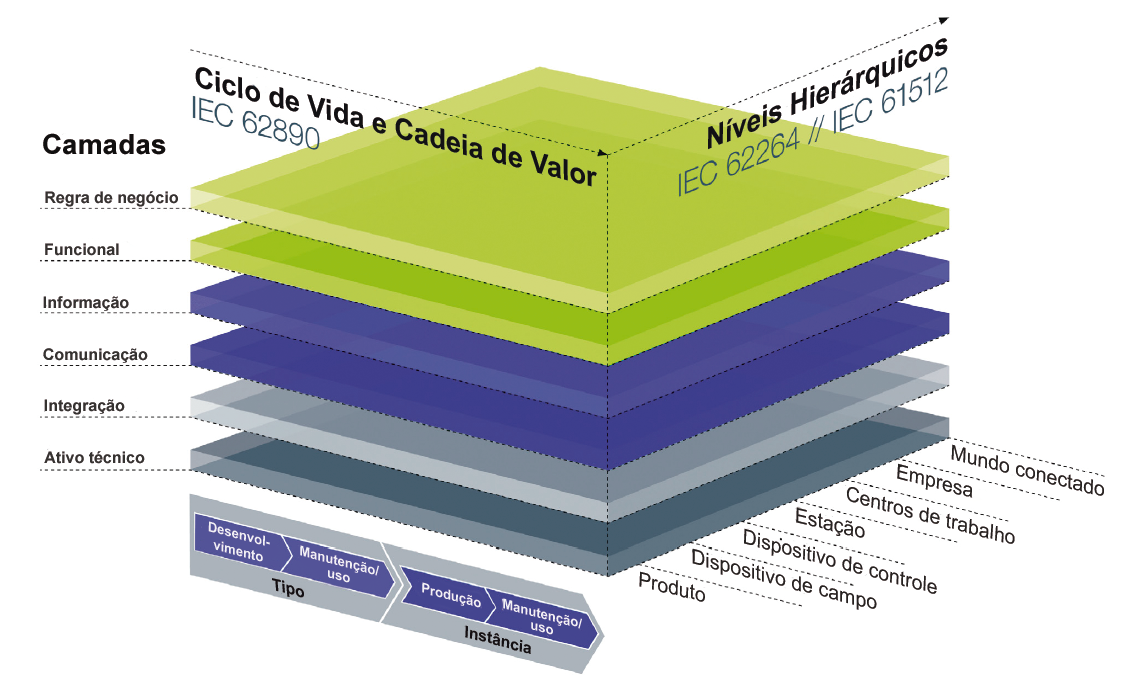
\includegraphics[width=1\textwidth]{rami4.png}
	\caption{Representação do RAMI4.0.}
	\label{fig:rami4}
	\fonte{\citeonline{adolphs2015rami} (adaptado).}
\end{figure}

O RAMI4.0, como um modelo de referência, é um elemento para padronização do projeto e implantação de aplicações em I4.0. O RAMI4.0 é uma padronização de linguagem e deve ser aceito e usado por todos os participantes para protótipo, desenvolvimento e validação.

\section{Motivação}
\label{sec:motivacao}

Os conceitos de I4.0 e MDP surgiram em 2011 \cite{kagermann2011industrie} e 2007 \cite{wahlster2007digitalmemory}, respectivamente. A área multidisciplinar de estudo envolvendo MDP e I4.0 surgiu em 2013 com o projeto SemProM \cite{wahlster2013semprom}, porém ainda quando I4.0 era um conceito abrangente e sem diretrizes concretas para sua implementação, o que ocorreria em 2013 por meio do documento de recomendações para implementação da iniciativa estratégia Industrie 4.0 \cite{kagermann2013recommendations}, antes da criação do modelo de arquitetura de referência para Indústria 4.0 (RAMI4.0), que seria divulgado em 2015 por um periódico alemão \cite{hankel2015rami}.

Alguns estudos como \citeonline{lasi2014industryfour} citam MDP como oportunidade de estudo e aplicação dentro da I4.0. Outros como \citeonline{weyer2015standardization} e \citeonline{paelke2014augmented} implementaram sistemas envolvendo ambos os conceitos, porém sem considerações sobre cadeia de valor.

Há estudos na área multidisciplinar de I4.0 e MDP, principalmente no meio acadêmico, empresarial e governamental alemão pelo fato de esses conceitos terem surgido na Alemanha. Porém nenhum trabalho até o presente momento relaciona o modelo de arquitetura de referência para a I4.0 (RAMI4.0) com a MDP. I4.0 e a MDP são conceitos altamente correlacionados, porém ainda não amplamente abordados em conjunto na literatura, o que aponta uma lacuna de conhecimento dentro de I4.0 a ser explorada.

Estudos sobre o RAMI4.0 são importantes no sentido de padronizar a implementação da I4.0 em empresas de diferentes negócios, garantindo assim a interoperabilidade dos serviços. O eixo ``Ciclo de Vida e Cadeia de Valor'' apresenta diretrizes para o correto planejamento da vida de um produto e sugere cenários para criação de valor perceptível ao produto/serviço. Integrar o conceito de MDP ao RAMI4.0 enriquece o nível de discussão sobre essa arquitetura de referência e dá mais robustez ao modelo para uma futura adoção generalizada por parte de empresas por todo o mundo.

A ``Plattform Industrie 4.0'' é uma das principais redes mundiais de discussão sobre I4.0 \cite{kagermann2013recommendations, acatech2014plattform, hartmut2019plattform}. O Conselho de Pesquisa da Plattform Industrie 4.0 é o comitê consultivo estratégico da Plattform Industrie 4.0 e identifica necessidades de pesquisa e ações em torno da I4.0. O comitê identificou e definiu quatro temas-chave de abordagens no setor tecnológico, econômico, metodológico e social/legal para se implementar com sucesso a I4.0 \cite{hirsch-kreinsen2019keythemes}, conforme mostrado na \autoref{fig:keythemes-i4}. Isso significa que os tópicos elencados são temas com alto potencial de otimização de rotinas e processos de produção existentes no cenário de I4.0.

\begin{figure}[htb]
	\centering
	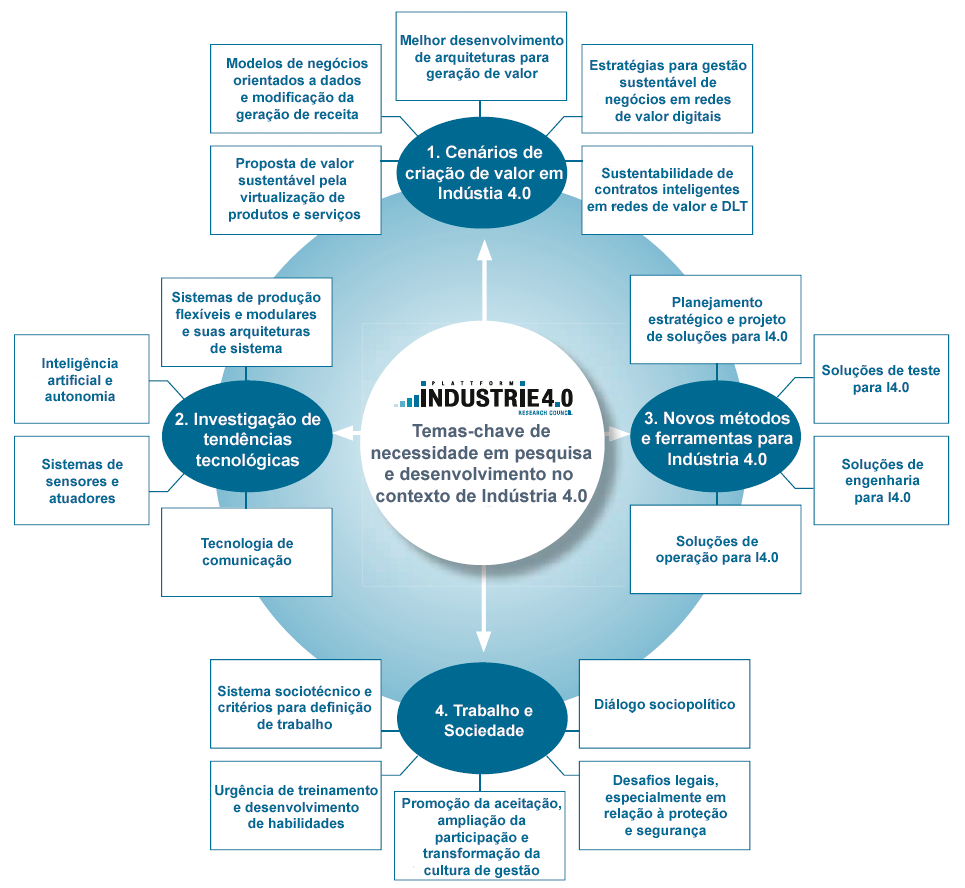
\includegraphics[width=1\textwidth]{keythemes-i4.png}
	\caption{Temas-chave de pesquisa e desenvolvimento em I4.0.}
	\label{fig:keythemes-i4}
	\fonte{\citeonline{hirsch-kreinsen2019keythemes} (adaptado).}
\end{figure}

Dentre os temas elencados na \autoref{fig:keythemes-i4}, destacam-se os subitens relacionados ao tópico ``Cenários de criação de valor em Indústria 4.0'' por estarem altamente relacionados ao RAMI4.0 e ao conceito de geração de valor por meio da MDP. O desenvolvimento de arquiteturas para geração de valor e a criação de negócios orientados a dados são temas de grande oportunidade dentro do cenário de I4.0, especialmente se considerando os métodos quantitativos de análise de dados já estabelecidos.

\section{Objetivos}
\label{sec:objetivos}

O objetivo geral e propósito do trabalho é a elaboração de uma arquitetura baseada no RAMI4.0 para o compartilhamento da memória digital do produto (MDP) ao longo da cadeia de suprimentos.

Para se alcançar o objetivo geral, este é desmembrado em escopos menores, representados pelos objetivos específicos. Os objetivos específicos do trabalho são:

\begin{itemize}
	\item \textbf{Integração da MDP ao Componente 4.0} (\autoref{sec:estrutura-aas}): para que a MDP possa ser compartilhada na I4.0, esta deve ser interoperável com os outros ativos presentes da indústria por meio do Componente 4.0, que é a junção de sua parte real e digital;
	\item \textbf{Levantamento de submodelos do produto e suas respectivas propriedades} (\autoref{sec:submodelos-produto}): as informações a serem compartilhadas pela cadeia de suprimentos devem estar encapsuladas em forma de submodelos e propriedades a fim de se adequarem ao RAMI4.0. Aqui são identificadas e classificadas informações relevantes do produto a serem compartilhadas;
	\item \textbf{Apresentação de considerações sobre a geração de valor por meio do compartilhamento da MDP ao longo ciclo de vida de um produto} (\autoref{sec:geracao-de-valor}): o compartilhamento de informações tem um potencial de geração de valor ao produto e ao negócio. Aqui são apontadas estas melhorias e como elas acontecem ao longo do ciclo de vida do produto;
	\item \textbf{Apresentação da arquitetura com seus componentes e operações} (\autoref{sec:componentes-e-operacoes}): a arquitetura proposta para o compartilhamento de informações é apresentada. Seus componentes e operações principais para o contexto da I4.0 principais são detalhados;
	\item \textbf{Demonstração da dinâmica de compartilhamento de informações por meio de serviços} (\autoref{sec:fluxo-de-fornecimento-de-servicos}): a dinâmica de compartilhamento de informações utilizando a arquitetura proposta é exemplificada por meio de cenários realísticos da indústria e cadeia de suprimentos;
	\item \textbf{Modelagem do fluxo de informações dentro das camadas do RAMI4.0} (\autoref{sec:mapeamento-das-operacoes}): a arquitetura é modelada para cada componente, cada interação e cada camada do RAMI4.0;
\end{itemize}

\section{Estrutura do trabalho}
\label{sec:estrutura}

O capítulo atual de introdução (\autoref{cha:introducao}) apresentou uma abordagem inicial dos conceitos que serão tratados ao longo do trabalho, a motivação e objetivos da pesquisa.

O \autoref{cha:fundamentos} apresenta a revisão bibliográfica realizada para a fundamentação dos conceitos necessários para a proposta da arquitetura de compartilhamento de informações do ativo. Cinco conceitos básicos são apresentados nesse capítulo: ``Indústria 4.0'', ``Logística \& Cadeia de Suprimentos'', ``Ciclo de vida do produto'', ``Memória digital do produto'', ``Arquitetura orientada a serviços'' e ``Modelagem de sistemas''.

O \autoref{cha:ciclo-de-vida} apresenta a proposta de integração da MDP ao Componente 4.0 para a interoperabilidade com outros componentes na Indústria 4.0. São apresentados os tipos de informações (submodelos e propriedades) a serem expostos e considerações sobre o impacto deste amplo compartilhamento da memória digital do produto ao longo da cadeia de suprimentos.

O \autoref{cha:arquitetura} apresenta os detalhes da arquitetura proposta baseada no RAMI4.0 para o compartilhamento de informações do ativo ao longo da cadeia de suprimentos. Neste capítulo é feita a modelagem da arquitetura e o mapeamento de cada um dos elementos desta arquitetura a cada um dos níveis do eixo Camadas do RAMI4.0.

Finalmente, no \autoref{cha:conclusao} são feitas as considerações sobre a pesquisa com comentários sobre os resultados alcançados e trabalhos futuros.
